%%%%%%%%%%%%%%%%%%%%%%%%%%%%%%%%%
%converted dpele to dc-tpcelec
\section{System Overview}
\label{sec:dp-tpcelec-overview}

The function of the \dword{dp} \dword{tpc} electronics system is to collect and digitize the signals from the \dwords{crp} (see chapter~\ref{ch:dp-crp}) and \dwords{pds} (see chapter~\ref{ch:dp-pds}). The first task is accomplished by the \dword{cro} and the second by the \dword{lro} subsystems. 

The design of the electronics system for the \dword{dune} \dword{dpmod} is the outcome of an R\&D program that began in 2006 and completed in 2016. This effort was initially targeted towards readout of very large liquid argon detectors and since 2011 it was focused on electronics optimization for \dword{dp} detector technology. The charge readout in a \dword{dp} \dword{tpc} offers some key advantages in comparison to that of a \dword{sp} detector. Most notably, while the \dword{dp} front-end electronics possesses the same low noise properties of the liquid argon-immersed cold electronics of \dword{sp} (\SI{110}{\kelvin} vs \SI{87}{\kelving} operation), the sub-system and all other electronics components for DP remain fully accessible for service, repair, replacement, or upgrade at any time during detector operations. This accessibility is achieved by integrating the analog front-end cards in dedicated feedthroughs (\dword{sftchimney}). This organization has also an impact on grouping of channels and their matching to the digitization electronics. The latter is decoupled from the analog stage and located on the roof of the cryostat at room temperature, which permits the use of low-cost high-speed networking technologies commonly employed in telecommunication industries (e.g., \dword{utca} standard). In addition, for the same detector mass the number of \dword{cro} channels is naturally smaller than for an \dword{sp} equivalent module (\num{153600} channels for \dword{dpmod} with \SI{3}{\mm} readout pitch to be compared \num{384000} channels for \dword{spmod} module with \SI{5}{\mm} readout pitch) as a consequence of a longer geometry of the drift volume. 

The design, finalized for \dword{dune} in 2016, went through several prototyping phases. The optimization aspects included matching the dynamics of the cryogenic charge amplifiers to the \dword{dp} readout structure and wide signal dynamic range as well as tailoring the digital front-end system accordingly. The \dword{snr} provided by \dword{dp} readout offers the possibility of performing efficient lossless compression at digitization stage without pedestal suppression (zero-suppression) while ensuring continuous acquisition and data transmission to \dword{daq} backend. A key criterion of the R\&D was to develop and build custom analog and digital electronics circuits, which are both cost-effective and easily scalable to meet the needs of a large-scale neutrino \dword{lar} detector. In 2016 we launched full-scale production of all of the components necessary for the charge readout of \dword{pddp}. In the same year a subset of the produced electronics was also deployed in the \dword{wa105} at CERN, a preliminary \dual \lartpc with an active volume  of \SI[product-units=power]{3x1x1}{m} (\dword{crp} area of \SI[product-units=power]{3x1}{m}), that took data in the summer and fall of 2017. The operation of the \dword{wa105} \cite{Aimard:2018yxp} gave early validation of the electronics  design choices and provided checks on various performance markers, such as noise. As an example, Figure~\ref{fig:dp-tpcelec-311-dqds-etaucorrected} shows a distribution of charge measured from reconstructed cosmic muon tracks for each of its collection views. After taking into account recombination, the average \dword{mip} charge loss expected in \lar is approximately \SI{10}{\femto\coulomb/\cm}. The effective gain of the \dword{crp} in the \dword{wa105} was between \numrange{3}{4}, which is lower than the target gain of \num{20} for \dword{dpmod} operation. Despite these lower-than-expected signals, the electronics system for \dword{cro} allowed us to perform measurements. 

\begin{dunefigure}[Charge distributions from cosmic ray tracks]{fig:dp-tpcelec-311-dqds-etaucorrected}
{Charge distributions from cosmic ray tracks for each collection view measured in \dword{wa105}  from \cite{Aimard:2018yxp}. View \num{0} (\num{1}) corresponds to \SI{3}{\meter} (\SI{1}{\meter}) long anode strips. In addition to the mean value of the distribution, each panel also shows the results---Most Probable Value (MPV) and widths of the Landau (Lwidth) and Gaussian (Gwidth)---obtained from a fit of the Landau function convoluted with a Gaussian distribution.}
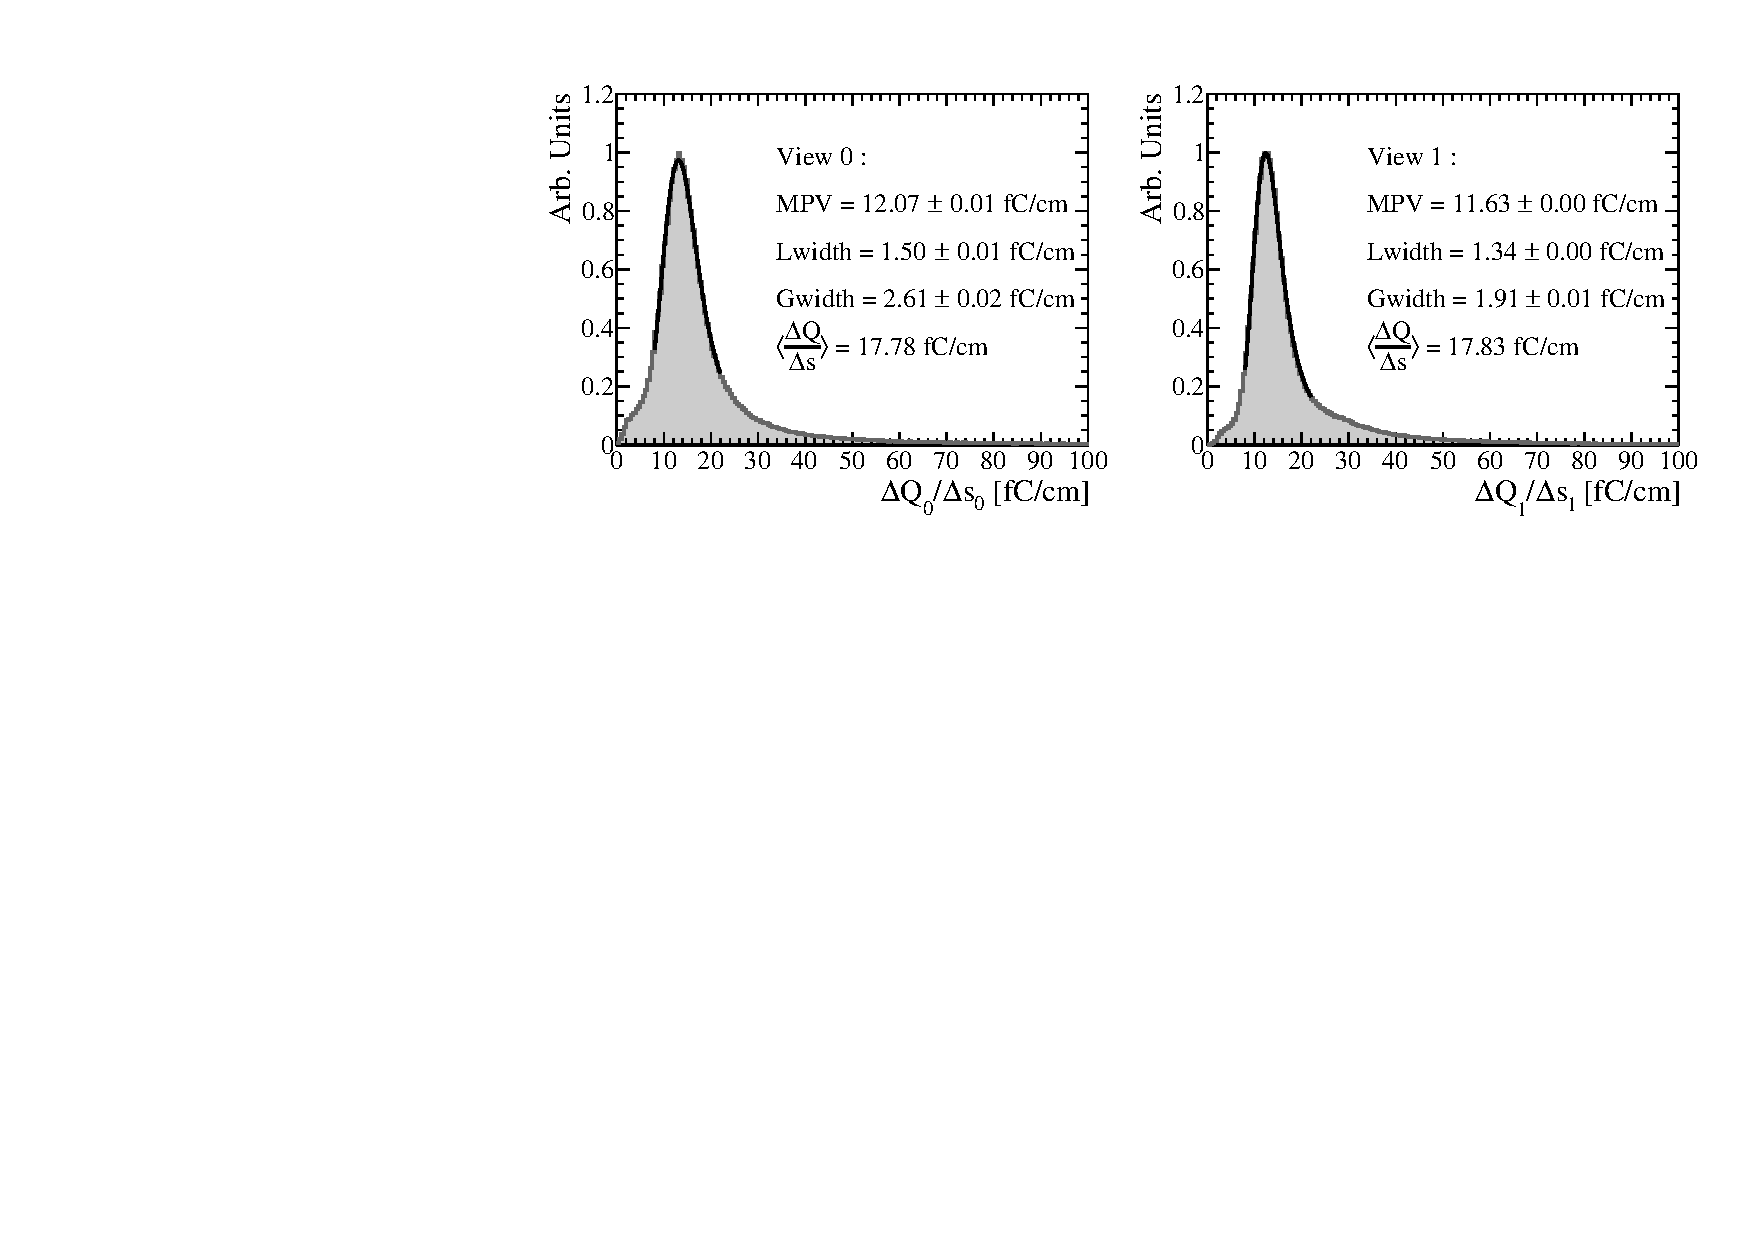
\includegraphics[width=0.8\textwidth]{dp-tpcelec-311-dqds-etaucorrected}
\end{dunefigure}

Measurements from \dword{wa105} demonstrator have assured us of the soundness of the existing design and all necessary elements of the \dword{cro} electronics system have been produced and tested for \dword{pddp}. Technical issues with \dwords{crp} have delayed the completion of \dword{pddp} preventing in turn the operation of the electronics. These issues have been largely resolved and cosmic ray data should be available by summer 2019. However, given past experience from \dword{wa105} and tests already performed on the production for \dword{pddp} we do not require particular additional inputs from \dword{pddp} operation for the design of the electronics system for \dword{dpmod} presented here. We additionally note that the \dword{dune} Executive Board has yet to formally ratify the set of specifications and requirements for \dword{dpmod}. This action should be taken in spring 2019; in the meantime this chapter has been developed using provisional specifications outlined in Section~\ref{ssec:dp-tpcelec-requir}.

\begin{comment}  Anne's not sure this is needed.
This chapter is organized as follows. In this section we provide an overview of the \dword{dp} \dword{tpc} electronics system and discuss design considerations. In Section~\ref{sec:dp-tpcelec-design}, we give detailed descriptions of the principal components. This is followed by the discussion of the production scheme, quality assurance and control, and calibration program in Section~\ref{sec:dp-tpcelec-production}. Section~\ref{sec:dp-tpcelec-transport} briefly covers the transportation and handling, while Section~\ref{sec:dp-tpcelec-intfc} describes interfaces to other detector systems. Details on the installation, integration, and commissioning of the \dword{dp} \dword{tpc} electronics system underground are provided in Section~\ref{sec:dp-tpcelec-install}. Sections~\ref{sec:dp-tpcelec-risks} and~\ref{sec:dp-tpcelec-safety} address risks and safety, respectively. Section~\ref{sec:dp-tpcelec-org} presents the organizational structure of the \dword{dp} \dword{tpc} electronics consortium, discusses schedule, and provides the estimates of the core costs. 
\end{comment}

%%%%%%%%%%%%%%%%%%%%%%%%%%%%%%%%%
\subsection{Introduction}
\label{ssec:dp-tpcelec-intro}

\begin{dunefigure}[Schematic layout of the \dword{dp} \dword{cro} subsystem]{fig:dp-tpcelec-crosystem-sketch}
{Schematic layout of the \dword{dp} \dword{cro} subsystem.}
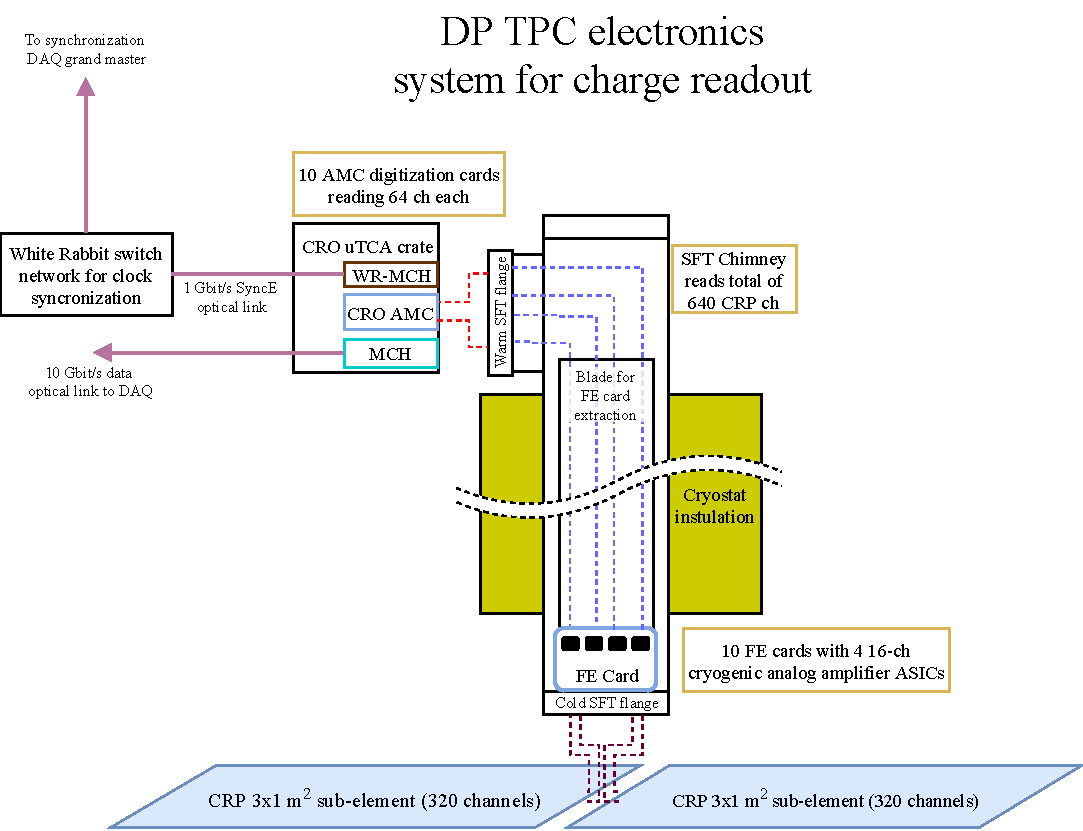
\includegraphics[width=0.6\textwidth]{dp-tpcelec-crosystem-sketch}
\end{dunefigure}

%The \dword{cro} electronics system, schematically illustrated in the Figure~\ref{fig:dp-tpcelec-crosystem-sketch}, is designed to provide continuous, non-zero-suppressed, and losslessly compressed digital signals by reading the charge collected on the \SI{3}{m} long \dword{crp} strips arranged in two collection views, all with a pitch of \SI{3.125}{mm}. The system consists of the \dword{fe} analog electronics operating at cryogenic temperatures that amplifies and shapes the signals from \dword{crp} strips and the digital electronics working in the warm environment outside the cryostat that digitizes the analog signals, compresses the resulting digitized data, and transmits them to the \dword{daq} system.  The cryogenic \dshort{fe} analog electronics uses an application-specific integrated circuit (\dword{asic}) chip with a large dynamic range (up to \SI{1200}{fC}) to cope with the charge amplification in the \dwords{crp}. The analog \dword{fe} cards are housed in dedicated \dwords{sftchimney} accessible from the outside even after the \dword{dpmod} is operating, thus removing any significant risks associated with their long-term survivability. The \dwords{sftchimney} are approximately \SI{2.3}{m} long stainless steel pipes that traverse the entire insulation layer of the cryostat allowing placement of the \dword{fe} electronics close to the \dwords{crp} to minimize cable capacitance (noise).  In addition, their metallic structure shields the \dword{fe} cards from any interference from the warm digital electronics and ambient environment. The analog signals are digitized by \dwords{amc}, which are housed in the commercial \dword{utca} crates on top of the cryostat near the \dwords{sftchimney}. 
The \dword{cro} electronics system, schematically illustrated in the Figure~\ref{fig:dp-tpcelec-crosystem-sketch}, is designed to read the charge collected on the \SI{3}{m} long \dword{crp} strips arranged in two collection views (all with a pitch of \SI{3.125}{mm}) and 
provide continuous, non-zero-suppressed, and losslessly compressed digital signals.  
The system consists of (1) the \dword{fe} analog electronics operating at cryogenic temperatures that amplifies and shapes the signals from \dword{crp} strips, and (2) the (warm) digital electronics external to the cryostat that digitizes the analog signals, compresses the resulting digitized data, and transmits them to the \dword{daq} system.  The cryogenic \dshort{fe} analog electronics uses an application-specific integrated circuit (\dword{asic}) chip with a dynamic range up to \SI{1200}{fC} to handle %cope with 
the charge amplification in the \dwords{crp}. The analog \dword{fe} cards are housed in dedicated \dwords{sftchimney} accessible from the outside at all times, thus removing any significant risks associated with their long-term survivability. The \dwords{sftchimney} are approximately \SI{2.3}{m} long stainless steel pipes that traverse the entire insulation layer of the cryostat, allowing placement of the \dword{fe} electronics close to the \dwords{crp} to minimize cable capacitance (noise).  In addition, their metallic structure shields the \dword{fe} cards from any interference from the warm digital electronics and ambient environment. The analog signals are digitized by \dwords{amc}, which are housed in the commercial \dword{utca} crates on top of the cryostat near the \dwords{sftchimney}. 

The \dword{cro} data are sampled at the rate of \SI{2.5}{MHz} with \SI{12}{bit} resolution. This frequency, %traditionally 
commonly used in \lartpc experiments, is well matched to the \SI{1}{\micro\second} pulse-shaping time of the \dword{fe} electronics and the detector response times determined by the electron drift velocity in the \lar. The corresponding sampling resolution along the drift coordinate is better than \SI{1}{\mm}. 

%The \dword{lro} electronics system, illustrated in the Figure~\ref{fig:dp-tpcelec-lrosystem-sketch},  collects and digitizes signals from the \dword{pds}, which consists of \dword{tpb}-coated \num{8}\,in \dwords{pmt} (Hamamatsu\footnote{Hamamatsu\texttrademark R5912-02-mod, \url{http://www.hamamatsu.com/}.} R5912-02-mod) beneath the \dword{tpc} cathode. The \dword{lro} electronics facilitate detecting the primary scintillation signals, which provide the absolute time reference for interaction events. The same electronics also enable recording light signals generated by photons from the so-called \textit{proportional scintillation component}, the light created by the electrons extracted and amplified in the gaseous phase. A fraction of this light can reach the \dwords{pmt} after traversing the entire detector volume. The \dword{lro} electronics, consisting of analog and digital stages, is housed in the \dword{utca} crates on top of the cryostat structure (like the \dword{cro} electronics). The \dword{lro} \dword{amc} card design shares a similar architecture with the \dwords{amc} for the charge readout. The \dword{lro} \dword{utca} crates are connected to specific \dword{lro} signal \fdth flanges on top of the cryostat (see chapter~\ref{ch:dp-pd}).
The \dword{lro} electronics system, illustrated in the Figure~\ref{fig:dp-tpcelec-lrosystem-sketch},  collects and digitizes signals from the \dword{pds}, which consists of \dword{tpb}-coated \num{8}\,in \dwords{pmt} (Hamamatsu\footnote{Hamamatsu\texttrademark R5912-02-mod, \url{http://www.hamamatsu.com/}.} R5912-02-mod) placed beneath the \dword{tpc} cathode. The \dword{pds} detects the primary scintillation signals, which provide the absolute time reference for interaction events. The same electronics also enables recording light signals generated by photons from what is called the proportional scintillation component, i.e., the light created by the electrons extracted and amplified in the gaseous phase. A fraction of this light can reach the \dwords{pmt} after traversing the entire detector volume. The \dword{lro} electronics, consisting of analog and digital stages, is housed in the \dword{utca} crates on top of the cryostat structure (as are the \dword{cro} electronics). The \dword{lro} \dword{amc} card design shares a similar architecture with the \dwords{amc} for the charge readout. Apart from a dedicated front-end stage, the \dword{lro} \dword{amc} inherits completely the well-tested circuitry and firmware of the \dword{cro} \dword{amc} and common operation environment. The \dword{lro} \dword{utca} crates are connected to specific \dword{lro} signal \fdth flanges on top of the cryostat (see chapter~\ref{ch:dp-pd}).

\begin{dunefigure}[Schematic layout of the \dword{dp} \dword{lro} subsystem]{fig:dp-tpcelec-lrosystem-sketch}
{Schematic layout of the \dword{dp} \dword{lro} subsystem.}
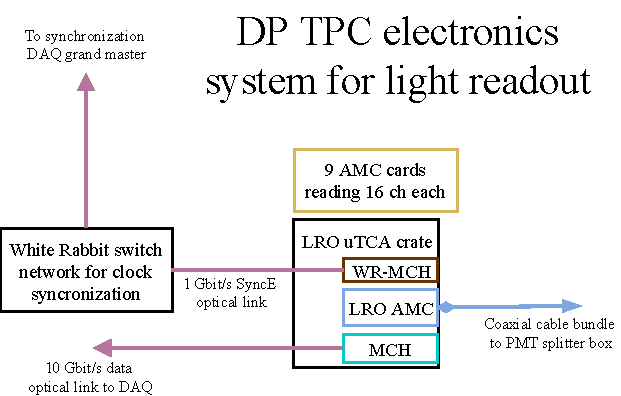
\includegraphics[width=0.6\textwidth]{dp-tpcelec-lrosystem-sketch}
\end{dunefigure}

Each \dword{utca} crate for either charge or light readout is connected to the \dword{daq} system via an optical fiber link that supports at least \SI{10}{Gbit/s}. Each crate also contains a \dword{wrmch} for time synchronization of the digital electronics. This timing slave unit is connected via \SI{1}{Gbit/s} optical fiber to a master node that serves as a synchronization reference for all connected slave nodes on the network. This system for time synchronization is built around the commercially available components from the \dword{wr} project\footnote{\url{https://www.ohwr.org/projects/white-rabbit}.} with \textit{ad hoc} hardware and firmware development. The system performs automatic and continuous self-calibrations to account for any propagation delays and can provide sub-\si{\nano\s} accuracy for timing synchronization.



%%%%%%%%%%%%%%%%%%%%%%%%%%%%%%%%%
\subsection{Design Considerations}
\label{ssec:dp-tpcelec-requir}

%The \dword{cro} electronics design covers the analog \dword{fe} cards containing pre-amplifier \dwords{asic} operating at cryogenic temperatures and digitization cards with the relevant system for their synchronization working in the warm environment outside of the cryostat. The system reads and digitizes signals from \num{153600} channels (per one \dword{dpmod}) and can continuously stream the collected and losslessly compressed data to the \dword{daq} without any zero suppression. 
The \dword{cro} electronics design includes the analog \dword{fe} cards (containing pre-amplifier \dwords{asic} operating at cryogenic temperatures) and digitization cards with their synchronization system installed outside of the cryostat. The system reads and digitizes signals from \num{153600} channels (the total number of \dword{cro} channels per one \dword{dpmod}) and can continuously stream the losslessly compressed data to the \dword{daq} with no zero suppression. 
%\fixme{one per what?} CLARIFIED
The% designed 
\dshort{cro} electronics system meets the following specifications: %fits the following requirements:
\fixme{to be replaced with a standardized table of specifications  }
\begin{itemize}
%\item{The \dword{cro} electronics must measure signals up to \SI{1200}{\femto\coulomb} without saturation; this has been optimized following \dword{mc} studies on the maximal occupancy per channel in shower events~\cite{WA105-TDR}. For a nominal \dword{crp} gain of \num{20}, a \dword{mip} signal should be approximately \SI{30}{fC}, the lowest limit that assumes a particle travelling horizontally with an azimuthal angle of \num{0} degrees, giving a maximal operational range of \num{40} \dwords{mip}.}
\item{The \dword{cro} electronics must measure signals up to \SI{1200}{\femto\coulomb} without reaching saturation. The system has reached this following \dword{mc} studies on the maximal occupancy per channel in shower events~\cite{WA105-TDR}. For a nominal \dword{crp} gain of \num{20}, a \dword{mip} signal from a particle travelling horizontally with an azimuthal angle of $\SI{0}{^\circ}$ (the lowest limit) should be approximately \SI{30}{fC}. This gives  a maximal operational range of \num{40} \dwords{mip}.}

\item{The electronic noise in the \dshort{cro} analog electronics must be \SI{< 2500}{e^{-}}. This condition can be derived from the requirement on the minimal \dword{s/n}, which should be more than \num{5}:\num{1} once the charge attenuation is taken into account. Given the maximum drift distance of \SI{12}{\meter}, the largest attenuation factor due to electro-negative impurities, assuming the \SI{3}{\milli\second} (minimally required) electron lifetime and the drift field of \SI{0.5}{\kilo\volt/\cm}, is \num{0.08}. The smallest \dword{mip} signal with the \dword{crp} effective gain of \num{20} is, therefore, \SI{2.5}{\femto\coulomb} (\SI{15600}{e^{-}}).}


%\item{The peaking time of the \dword{fe} analog amplifiers must be \SI{1}{\micro\second} because optimal vertex resolution is necessary. This resolution is determined in turn by the single track resolution and the power to separate two or more tracks close to one another.}
\item{To acheive optimal vertex resolution, the peaking time of the \dword{fe} analog amplifiers must be \SI{1}{\micro\second}. The optimal resolution is determined by the single track resolution and the separability of two or more tracks close to one another.}

\item{The sampling frequency must be \SI{2.5}{\MHz} to match the peaking time of the \dword{fe} electronics.}

\item{The power dissipated by the \dword{fe} analog electronics must be below \SI{50}{\milli\watt/channel} to minimize heat input to the cryostat volume.}

\item{The \dword{fe} analog electronics must be replaceable without contaminating the main \lar volume to guarantee the long-term reliability of the system.}

\item{The \dword{adc} resolution must be such that the noise is at the level of an \dword{adc} count, given a dynamic range wide enough to match the response of the \dword{fe} amplifier. This can be achieved with a \num{12} bit \dword{adc}.} 

\item{%The digital electronics placed outside the cryostat in the warm environment must be capable of 
The warm digital electronics must accommodate standard industrial components and solutions to keep costs low and to benefit from technological evolution, e.g., higher network speeds.}
\end{itemize}
As described in subsequent sections, %the performance of the final system is significantly better than many of the listed requirements. 
the system exhibits significantly better performance than set forth in the requirements.

%The magnitude of the noise also affects the quality of the lossless compression of the raw data. The system achieves a %A 
%compression factor of approximately \num{10} %is achieved 
%with an \rms noise level less than \SI{1}{\dword{adc}}. To give an idea of the compression efficiency dependency on the noise level, a compression factor of four is obtained with noise at approximately \SI{1.5}{\dword{adc}} counts. 
The (lossless) data compression efficiency is dependent on the noise level. A compression factor of four is obtained with noise at approximately \SI{1.5}{\dword{adc}} counts, and  
 a compression factor of approximately \num{10} 
with an \rms noise level less than \SI{1}{\dword{adc}}. 


%The primary objective of the \dword{lro} system is to detect signals from a minimum of one \phel on one \dword{pmt}, giving a precise timestamp that can be used in conjunction with the charge signals to determine the absolute event time ($T_0$). Precise measurements of \dword{lro} signal charge allow  continual monitoring of the \dword{pmt} gain at a single \phel level, as well as determining the number of photons in each scintillation event.  In addition, an \dword{adc}  continuously streams data, downsampled to \SI{400}{ns} as for the \dword{cro} signals,  which, among other things, allows the scintillation time profile to be measured. The \dword{lro} system also reads \num{20} channels from reference SiPM sensors from the \dword{pd} calibration system.
The  \dword{lro} system must detect signals from a minimum of one \phel on one \dword{pmt}, giving a precise timestamp that can be used in conjunction with the charge signals to determine the absolute event time ($t_0$). Precise measurements of \dword{lro} signal charge at a single \phel level allow continual monitoring of the \dword{pmt} gain, as well as determination of the number of photons in each scintillation event. 
%\fixme{how does the precision of the measurements connect to the continual aspect of the monitoring?} -> PMT gain can be continuosly measured/monitored from single photoelectron events; the sentence is correct.
The continuous \dword{adc} streaming of data, downsampled to \SI{400}{ns} as for the \dword{cro} signals, allows measurement of the scintillation time profile. The \dword{lro} system also reads \num{20} channels from reference \dword{sipm}  sensors from the \dword{pd} calibration system.


The cryogenic analog electronics for the \dword{cro} is housed in the dedicated \dwords{sftchimney}. Its design enables access to the \dword{fe} card so that it can be replaced without contaminating the pure \lar in the main cryostat volume. The chimneys have a cooling system that can control the temperature around the \dword{fe} cards to roughly \SI{110}{\kelvin} to reach their optimal noise level; this compensates for the heat input from the chimneys into the cryostat volume. 

The digital electronics for both charge and light readout is in the warm environment on the top of the cryostat support structure. % and is easily accessible. 
This removes any constraints associated with  accessibility and operation in cryogenic environments, allowing use of standard components and industrial solutions in the design. Digital electronics must be continuously and automatically synchronized to more than \SI{400}{\nano\s} to ensure the correct temporal alignment of the \dword{adc} samples from all of the readout channels. This is a minimal requirement dictated by a sampling rate of \SI{2.5}{\MHz}.  

%\fixme{I just noted that the header in the PDF reads LIST OF TABLES.} 
Key parameters for the electronics system design are summarized in Table~\ref{tab:dp-tpcelec-physicsparams}. 

\begin{dunetable}
[Key parameters for the TPC electronics system design]
{lr}
{tab:dp-tpcelec-physicsparams}
{Key parameters for the  TPC electronics system design %. The values given for the total number of channels and data rate are 
for one \dword{dpmod}.}   
Parameter & Value  \\ \toprowrule
  \dword{cro} channels    & \dpnumcrpch           \\ \colhline
  \dword{cro} continuous sampling rate & \SI{2.5}{\MHz}\\ \colhline
  \dword{cro} \dword{adc} resolution & \num{12}\,bit           \\ \colhline
  \dword{cro} data compression factor   & \num{10}    \\ \colhline 
  \dword{cro} data flow  & \num{430}\,Gibit/s          \\ \colhline 
  \dword{lro} channels       & \dpnumpmtch             \\ \colhline
  \dword{lro} continuous sampling rate & \SI{2.5}{\MHz} \\ \colhline
  \dword{lro} \dword{adc} resolution & \num{14}\,bit            \\ \colhline
  \dword{lro} data compression factor  & \num{1}       \\ \colhline
  \dword{lro} data flow   & \num{24}\,Gibit/s          \\ 
\end{dunetable}


%%%%%%%%%%%%%%%%%%%%%%%%%%%%%%%%%
\subsection{Scope}
\label{ssec:dp-tpcelec-scope}


The scope of the \dword{tpc} electronics system covers procurement, production, testing, validation, installation, and commissioning of all components necessary to ensure the complete readout of the charge and light signals from a given \dword{dpmod}. This includes 
\begin{itemize}
\item{Cryogenic analog \dword{fe} cards for charge readout;}
\item{\dword{amc} cards for charge and light readout;}
\item{The \dword{wrmch} cards for \dword{amc} clock synchronization;}
\item{\dword{utca} crates;}
\item{Switches for the \dword{wr} network;}
\item{\dwords{sftchimney};}
\item{\dword{lv} power supplies, distribution, and filtering system for the \dword{fe} cards;}
\item{Flat cables connecting the \dword{fe} cards to the warm flange interface of the \dwords{sftchimney};}
\item{VHDCI cables connecting the warm flange interface of the \dwords{sftchimney} to \dwords{amc}.}
\end{itemize}

The total number of components to be procured to instrument one \dword{dpmod} are given in Table~\ref{tab:dp-tpcelec-num-components}.

\begin{dunetable}
[Numbers for \dual electronics components to procure]
{lr} {tab:dp-tpcelec-num-components}
{Numbers for \dual electronics components to procure for one \dword{dpmod}.}
Name & Number  \\ \toprowrule
\dword{cro} cryogenic \dwords{asic} (\num{16} ch) & \num{9600} \\ \colhline
\dword{cro} cryogenic analog \dword{fe} cards (\num{64} ch) & \num{2400} \\ \colhline
\dword{cro} \dwords{amc} & \num{2400} \\ \colhline
\dwords{sftchimney} & \num{240} \\ \colhline
Flat cables for \dword{sftchimney} (\num{68} ch) & \num{2400} \\ \colhline
Flat cables for \dword{sftchimney} (\num{80} ch) & \num{2400} \\ \colhline
VHDCI cables (\num{32} ch) & \num{4800} \\ \colhline
\dword{lro} \dwords{amc} with analog \dword{fe} & \num{45} \\ \colhline
\dword{utca} crates & \num{245} \\ \colhline
\dword{wrmch} units & \num{245} \\ \colhline
WR switches (\num{18} ports) & \num{16} \\ 
\end{dunetable}

